\documentclass{article}
\usepackage{fancyhdr, graphicx, multicol}

\title{\huge \textbf{Hog Language Reference}}
\author{Jason Halpern\\ Samuel Messing\\ 
        Benjamin Rapaport \\  Kurry Tran \\ Paul Tylkin}

\begin{document}
\maketitle
\newpage

\section{Introduction}
\label{sec:introduction}

As data sets have grown in size, so have the complexities of dealing with them.
For instance, consider wanting to generate counts for all the words in \emph{War
and Peace} by means of distributed computation. Writing in Java and using Hadoop
MapReduce (TM), a simple solution takes over 50 lines of code, as the programmer
is required to specify intermediate objects not directly related to the desired
computation, but required simply to get Hadoop to function properly. Our goal is
to produce a language that can express the same computation in about 10 lines.

\subsection{The MapReduce Framework}
\label{sub:mapreduce}

With the explosion in the size of datasets that companies have had to manage in
recent years there are many new challenges that they face. Many companies and
organizations have to handle the processing of datasets that are terabytes or even
petabytes in size. The first challenge in this large-scale processing is how to
make sense of all this data. More importantly, how can they process and manipulate
the data in a time efficient and reliable manner. The second challenge is how they
handle this across their distributed systems. Writing distributed, fault-tolerant
programs requires a high level of expertise and knowledge of parallel systems.

In response to this need, a group of engineers at Google developed the MapReduce
framework in 2004. This high-level framework can be used for of a variety of
tasks, including handling search queries, indexing crawled documents and
processing logs. The software framework was developed to handle computations on
massive datasets that are distributed across hundreds or even thousands of
machines. The motivation behind MapReduce was to create a unified framework that
abstracted away many of the low level details from programmers, so they would not
have to be concerned with how the data is distributed, how the computation is
parallelized and how all of this is done in a fault tolerant manner.

The MapReduce framework partitions input data across different machines, so that
the computations are initially performed on smaller sets of data distributed
across the cluster. Each cluster has a master node that is responsible for
coordinating the efforts among the slave nodes. Each slave node sends periodic
heartbeats to the master node so it can be aware of progress and failure. In the
case of failure, the master node can reassign tasks to other nodes in the cluster.
In conjunction with the underlying MapReduce framework created at Google, the
company also had to build the distributed Google File System (GFS). This file
system ``allows programs to access files efficiently from any computer, so
functions can be mapped everywhere.'' GFS was designed with the same goals as
other distributed file systems, including ``performance, scalability, reliability
and availability.'' Another key aspect of the GFS design is fault tolerance and
this is achieved by treating failures as normal and optimizing for ``huge files
that are mostly appended to and then read.''

Within the framework, a programmer is responsible for writing both Map and Reduce
functions. The map function is applied to all of the input data ``in order to
compute a set of intermediate key/value pairs.'' In the map step, the master node
partitions the input data into smaller problems and distributes them across the
worker nodes in the cluster. This step is applied in parallel to all of the input
that has been partitioned across the cluster. Then, the reduce step is responsible
for collecting all the processed data from the slave nodes and formatting the
output. The reduce function is carried out over all the values that have the same
key such that each key has a single value. which is the answer to the problem
MapReduce is trying to solve. The output is done to files in the distributed file
system.

The use of ``a functional model with user-specified map and reduce operations
allows (Google) to parallelize large computations easily and to use re-execution
as the primary mechanism for fault tolerance.'' A programmer only has to specify
the functions described above and the system handles the rest of the details.
Figure \ref{fig:map_reduce_overview} illustrates the execution flow of a MapReduce
program.

\begin{center}
\begin{figure}
  \label{fig:map_reduce_overview}
  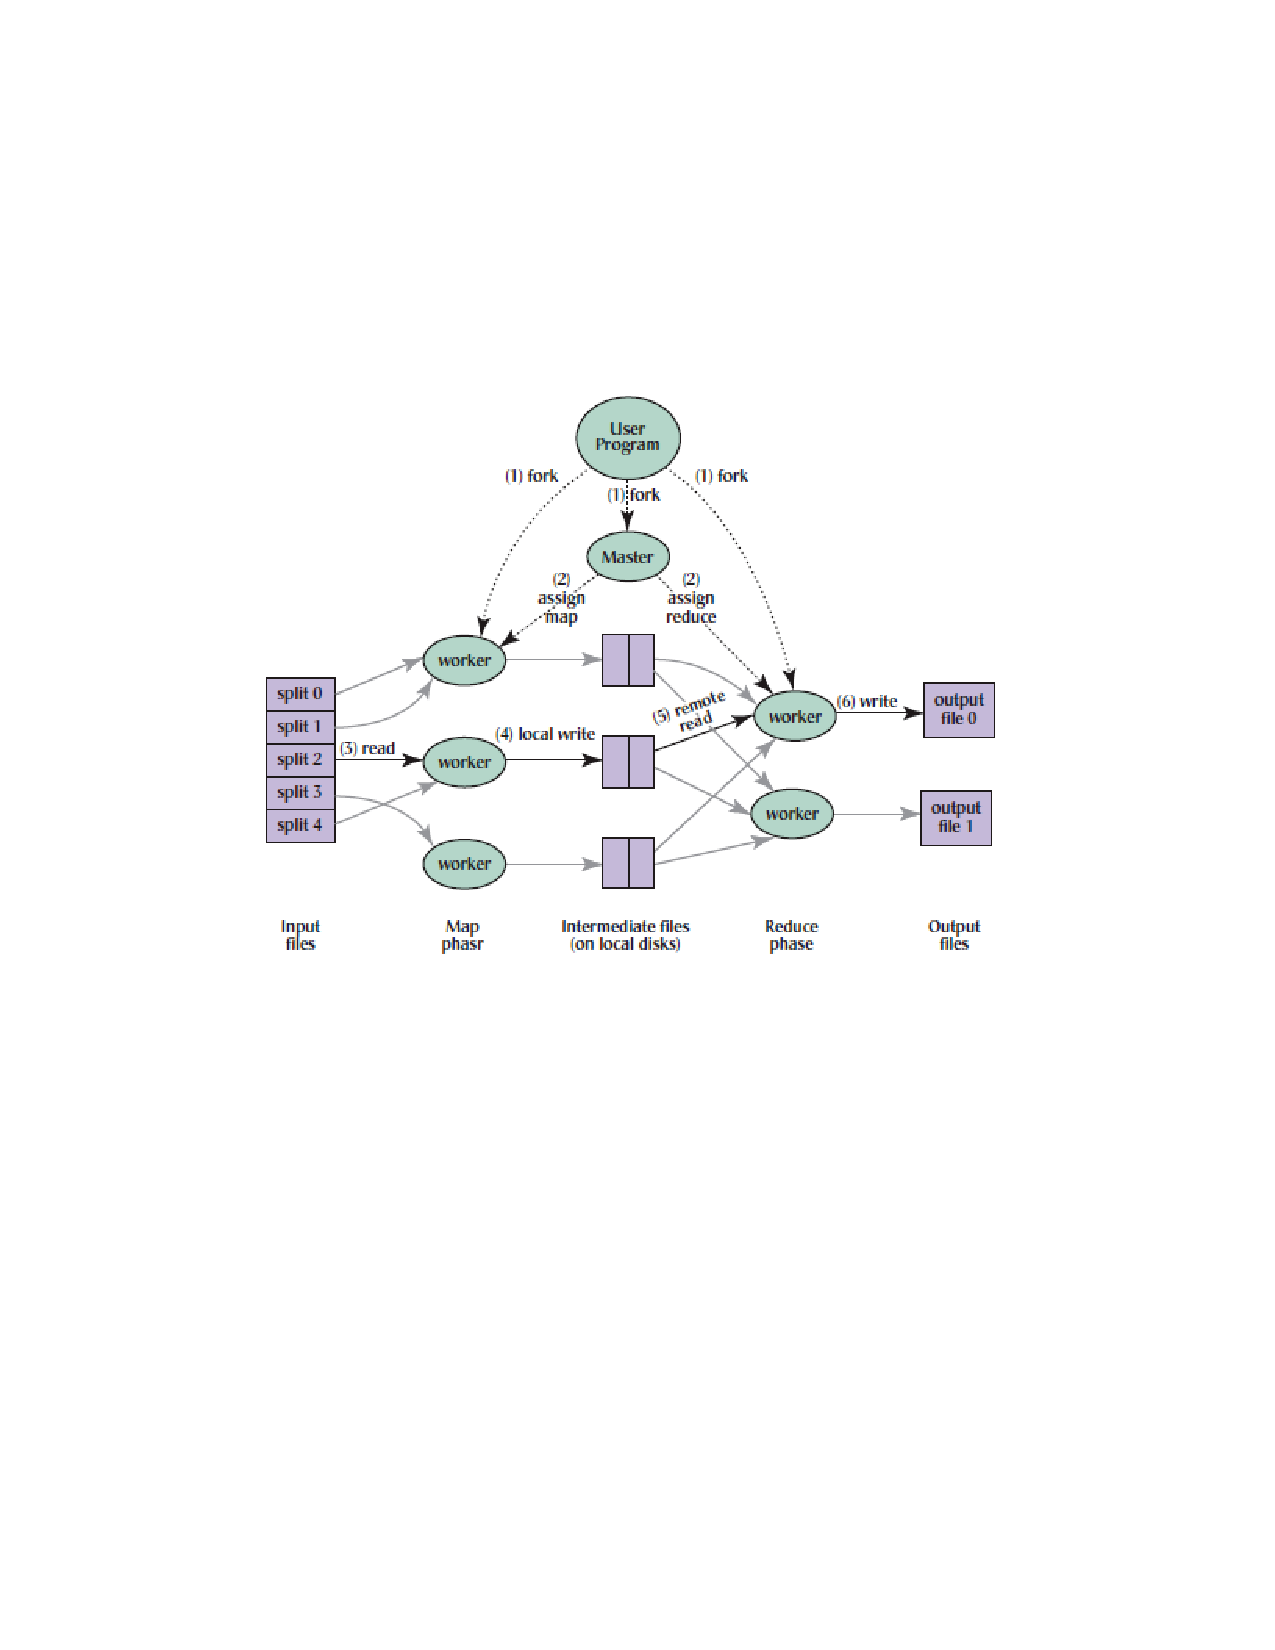
\includegraphics[width=0.85\textwidth]{img/map_reduce_overview.pdf}
  \caption{Overview of the Map Reduce program}
\end{figure}
\end{center}

\subsection{The Hog Language}
\label{sub:hog_language}

Hog is a \textbf{data-oriented}, \textbf{high-level}, scripting language for
creating MapReduce programs. Used alongside Hadoop, Hog enables users to
efficiently carry out \textbf{distributed} computation. Hadoop MapReduce is an
open-source implementation of the MapReduce framework, which is especially useful
for working with large data sets. While it is possible to write code to carry out
computations with Hadoop directly, the framework requires users to specify
low-level details that are often irrelevant to their desired goal.

By building a scripting language on top of Hadoop, we aim to simplify the process.
Built around a \textbf{simple} and highly \textbf{readable} syntax, Hog will let
users focus on what computations they want done, and not how they want to do them.
Hog takes care of all the low-level details required to run computations on
Hadoop’s distributed network. All a user needs to do is tell Hog the location of
their valid Hadoop instance, and Hog will do the rest.

We intentionally have restricted the scope of Hog to deal with specific problems.
For example, Hog's collection objects can only contain primitive types (preventing
such data structures as lists of lists). Also, Hog only supports reading and
writing plaintext files. While these limitations sacrifice the generality of the
language, they promote ease of use.

\subsubsection{Guiding Principles} % (fold)
\label{ssub:guiding_principles}

The guiding principles of Hog are:

\begin{itemize}
  \item Anyone can MapReduce
  \item Brevity over verbosity
  \item Simplicity over complexity
\end{itemize}


% subsubsection guiding_princples (end)

\subsection{The \lq\lq Ideal \rq\rq Hog User} % (fold)
\label{sub:the_ideal_hog_user}

Hog was designed with a particular user in mind: one that has already learned the basics of programming in a different
programming language (such as Python or Java), but is inexperienced with distributed computation and can benefit from a highly structured framework for writing MapReduce programs. The language was designed with the goal of making learning how to write MapReduce programs as easy as possible. However, the user should be adept with programming concepts such as program structure, control flow (iteration and conditional operators), evaluation of boolean expressions, etc.

% subsection the_ideal_hog_user (end)

\section{Program Structure} % (fold)
\label{sec:program_structure}

\subsection{Overall Structure} % (fold)
\label{sub:overall_structure}

Every Hog program consists of a single source file with a ‘.hog’ extension. This
source file must contain three sections: \tt @Map\rm, and \tt @Reduce\rm, and
\tt @Main \rm and can also include an optional \tt @Functions \rm section. These
sections must be included in the following order:

\begin{verbatim}
    @Functions {
      .
      .
      .
    }
    @Map <type signature> {
      .
      .
      .
    }
    @Reduce <type signature> {
      .
      .
      .
    }
    @Main {
      .
      .
      .
    }
\end{verbatim}

% section overall_structure (end)

\subsection{\tt @Functions\rm} % (fold)
\label{sub:tt_functionsrm}

At the top of every Hog program, the programmer has the option to define functions
in a section called \tt @Functions\rm. Any function defined in this section can be
called from any other section of the program, including \tt @Map\rm, \tt
@Reduce\rm, and \tt @Main \rm and can also be called from other functions defined
in the \tt @Functions \rm section. The section containing the functions begins
with the keyword \tt @Functions \rm on its own line, followed by the function
definitions.

Function definitions have the form:

\begin{quotation}
  \tt @Functions \{ \rm \\
  \indent \emph{type functionName(parameterList)} \tt \{ \rm \\
  \indent \indent \emph{expressionList} \\
  \indent \tt \}\}
\end{quotation}

The return-type can be any valid Hog type. The rules regarding legal function-names
are identical to those regarding legal variable identifiers. Each parameter in the
parameter-list consists of a valid Hog type followed by the name of the parameter,
which must also follow the naming rules for identifiers. Parameters in the
parameter-list are separated by commas. The @Functions section ends when the next
Hog section begins.

A complete example of an @Functions section:

\begin{verbatim}
    @Functions {
      int min(int a, int b) {
        if (a < b) {
          return a
        } else {
          return b
        }
      }

      list<int> reverseList(list<int> oldList) {
        list<int> newList()
        for (int i = oldList.len()-1; i >= 0; i--) {
          newList.append(oldList.get(i))
        }
        return newList
      }
    }
\end{verbatim}

Function names can be overloaded as long as the function definitions have different
signatures (i.e. parameter lists different in types and/or length). Additionally,
user-defined functions can make reference to other user-defined functions.

% section tt_functionsrm (end)

\subsection{\tt @Map \rm} % (fold)
\label{sub:tt_map_rm}

The map function in a MapReduce program takes as input key-value pairs, performs
the appropriate calculations and procedures, and emits intermediate key-value
pairs as output. Any given input pair may map to zero, one, or multiple output
pairs. The \tt @Map \rm section defines the code for the map function.

The \tt @Map \rm header must be followed by the signature of the map function, and
then the body of the map function as follows:

\begin{quotation}
  \tt @Map ( \rm \emph{type identifier, type identifier} \tt ) -> ( \rm \emph{type, type} \tt ) \{ \\
  \indent \indent . \\
  \indent \indent . \\
  \indent \indent . \\
  \indent \tt \} \rm
\end{quotation}

The first \tt type identifier \rm defines the \emph{\textbf{key}} and the second
defines the \emph{\textbf{value}} of the input key-value pair to the \tt @Map \rm
function. The identifiers specified for the key and value can be made reference to
later within the \tt @Map \rm block. The \tt @Map \rm signature is followed by an
arrow and another key-value pair, defining the types of the output of the map
function. Notice that identifiers are not specified for the output key and value
(said to be \emph{unnamed}), as these pairs are only produced at the end of the
map function. Also note that any code written in the same scope after an \tt
emit() \rm call will be \textbf{\emph{unreachable}}, and will cause a compile-time
\tt UnreachableCodeException\rm.

The map function can include any number of calls to \tt emit()\rm, which outputs
the resulting intermediate key-value pairs for use by the function defined in the
\tt @Reduce \rm section. The types of the values passed to the \tt emit() \rm
function must agree with the signature of the output key-value pair as defined in
the \tt @Map \rm type signature. All output pairs from the map function are
subsequently grouped by key by the framework, and passed as input to the \tt
@Reduce \rm function.

Currently, the only configuration available is for a file to be passed into the map
function one line at a time, with the line of text being the value, and the
corresponding line number as the key. This requires that the input key/value pair
to the map function is of type \tt (int key‐name,text value‐name)\rm. Extending
this to allow for other input formats is a future goal of the Hog language.

The following is an example of a complete \tt @Map \rm section for a program that
counts the number of times each word appears in a set of files. The map function
receives a single line of text, and for each word in the line (as delineated by
whitespace), it emits the word as the key with a value of one. By emitting the word
as the key, we can allow the framework to group by the word, thus calling the
reduce function for every word.

\begin{verbatim}

  @Map: (int lineNum, text line)  ->  (text, int) {
    foreach word in line.tokenize(" ") {
      emit(word, 1)
    }
  }

\end{verbatim}


% section tt_map_rm (end)

\subsection{\tt @Reduce \rm} % (fold)
\label{sub:tt_reduce_rm}

The reduce function in a MapReduce program takes a list of values that share the
same key, as emitted by the map function, and outputs a smaller set of values to
be associated with another key. The input and output keys do not have to match,
though they often do.

The setup for the reduce section is similar to the map section. However, the input
value for any reduce function is always an iterator over the list of values
associated with its key. The type of the key must be the same as the type of the
key emitted by the map function. The iterator must be an iterator over the type of
the values emitted by the map function.

\begin{quotation}
  \tt @Reduce ( \rm \emph{type identifier, type identifier} \tt ) -> ( \rm \emph{type, type} \tt ) \{ \\
  \indent \indent . \\
  \indent \indent . \\
  \indent \indent . \\
  \indent \tt \} \rm
\end{quotation}

As with the map function, the reduce function can emit as many key/value pairs as
the user would like. Any key/value pair emitted by the reduce function is recorded
in the output file.

Below is a sample \tt @Reduce \rm section, which continues the word count example,
and follows the \tt @map \rm sample introduced in the previous section.

\begin{verbatim} 

     @Reduce: (text word, iter<int> values) -> (text, int) {                   
            int count = 0                                                                  while (values.hasNext()) {                                                          count = count + values.getNext()                              
            }                                                                              emit(word, count)                                                        }  

\end{verbatim} 

% subsection tt_reduce_rm (end)

\subsection{\tt @Main \rm} % (fold)
\label{sec:tt_main_rm}

The @Main section defines the code that is the entry point to a Hog program. In
order to run the map reduce program defined by the user in the previous sections,
@Main must contain a call to the system-level built-in function mapReduce(). Other
arbitrary code can be run from the @Main section as well. Currently, @Main does
not have access to the results of the map reduce program resulting from a call to
mapReduce(). Therefore, it is quite common for the @Main section to contain the
call to mapReduce() and nothing else.

Below is a sample @Main section which prints to the standard output and runs a map reduce job.

\begin{verbatim}
    @Main {
          print("Starting mapReduce job.\n")
          mapReduce()
          print("mapReduce complete.\n")
    }
\end{verbatim}


% subsection tt_main_rm (end)

% section program_structure (end)

\section{Lexical Conventions} % (fold)
\label{sec:lexical_conventions}

\subsection{Tokens} % (fold)
\label{sub:tokens}

The classes of tokens include the following: identifiers, keywords,
constants, string literals, operators and separators. Blanks, tabs, newlines and
comments are ignored. If the input is separated into tokens up to a given
character, the next token is the longest string of characters that could represent
a token.

% subsection tokens (end)

\subsection{Comments} % (fold)
\label{sub:comments}

Multi-line comments are identified by the enclosing character sequences \tt \#\{ \rm and \tt \}\#\rm. Anything within these
enclosing characters is considered a comment, and is completely ignored by the compiler. For example,

\begin{verbatim}
    int i = 0
    #{ these are block
        comments and are ignored
         by the compiler }#
    i++
\end{verbatim}

In the above example, the text \tt these are block comments \textbackslash n comments and are ignored \textbackslash n by the
complier \rm are completely ignored during compilation. Compilation goes directly from the line \tt int i = 0 \rm to the line
\tt i++\rm.

Single-line comments are defined to be strings of text included between a '\tt
\#\rm' symbol on the left-hand side an a newline character ('\tt\textbackslash
n\rm') on the right-hand side.

% subsection comments (end)

\subsection{Identifiers} % (fold)
\label{sub:identifiers}

A valid identifier in Hog is a sequence of contiguous letters, digits, or
underscores, which are used to distinguish declared entities, such as 
methods, parameters, or variables from one another. A valid identifier also
provide a means of determining scope of an entity, and helps to determine whether
the same valid identifier in another scope refers to the same entity. The first
character of an identifier must not be a digit. Valid identifiers are case sensitive
so foo is not the same identifier as Foo.

% section identifiers (end)

\subsection{Keywords} % (fold)
\label{sub:keywords}

The reserved words of Hog are a superset of the reserved words of Java, since
Hadoop scripts compile into runnable Java code. The following words are reserved
for use as keywords, and may not be redefined by a programmer:

\begin{multicols}{4}
\tt
\begin{itemize}
  \item[] @functions
  \item[] @main
  \item[] @map
  \item[] @reduce
  \item[] and
  \item[] bool
  \item[] break
  \item[] case
  \item[] catch
  \item[] default
  \item[] dict
  \item[] else
  \item[] elseif
  \item[] emit
  \item[] final
  \item[] for
  \item[] foreach
  \item[] hadoop
  \item[] if
  \item[] in
  \item[] instanceof
  \item[] int
  \item[] iter
  \item[] list
  \item[] map
  \item[] not
  \item[] or
  \item[] real
  \item[] return
  \item[] switch
  \item[] text
  \item[] throw
  \item[] try
  \item[] void
  \item[] while
\end{itemize}
\rm
\end{multicols}

% subsection keywords (end)

\subsection{Constants} % (fold)
\label{sub:constants}

There are different kinds of constants, corresponding to each of the primitive data types in Hog. Once a variable has been declared a constant, its type and value cannot be changed. To declare a constant, use the following notation:

   final type variableName value

\begin{verbatim}
constants can be of the following types:
   int
   real
   bool
   text  
\end{verbatim}

Example:
{\tt int} constants would be declared as such:
     final int rate 100

% subsection constants (end)

\subsection{String Literals} % (fold) \label{sub:string_literals} A string literal
consists of a sequence of zero of more contiguous characters enclosed in double
quotes, such as "hello". A string literal can also contain escape characters such
as "\textbackslash n" for the new line character or "\textbackslash t" for the tab
character. A string literal has a String type has many of the same builtin
functions as the String class in Java. String literals are constant and their
values cannot be changed after they are created. String literals can be
concatenated with adjacent string literals by use of the "+" operator and are then
converted into a single string. Hog implements concatention by use of the Java
StringBuilder(or StringBuffer) class and its append method. All string literals in
Hog programs are implemented as instances of the String class, and then are mapped
directly to the equivalent String class in Java.

% subsection string_literals (end)

\subsection{Variable Scope} % (fold)
\label{sub:variable_scope}

Hog implements what is generally referred to as lexical scoping or block scope. An
identifier is valid within its enclosing block. The identifier is also value for
any block nested within its enclosing block.

% subsection variable_scope (end)

% section lexical_conventions (end)

\section{Syntax Notation} % (fold)
\label{sec:syntax_notation}

In the syntax notation used throughout the Hog manual, different syntactic
categories are noted by italic type, and literal words and characters are in
typewriter style.

% sec syntax_notation (end)

\section{Types} % (fold)
\label{sec:types}

\subsection{Basic Types} % (fold)
\label{sub:basic_types}

The basic types of Hog include \tt int \rm (integer numbers in base 10, 64 bytes
in size), \tt real \rm (floating point numbers, 64 bytes in size), \tt bool
\rm(boolean values, true or false) and \tt text \rm (Strings, variable in size).
Unlike most languages, Hog includes no basic character type. Instead, a programmer
makes use of \tt text\rm s of size 1.

\emph{Implementation details} Hog’s primitive types are not so primitive. They are
in fact wrappers around Hadoop classes. For instance, Hog’s \tt int \rm type is a
wrapper around Hadoop's \tt IntWritableclass\rm. The following lists for every
primitive type in Hog the corresponding Hadoop class that the type is built on top
of:

\begin{center}
\begin{tabular}{|c|c|}
    \hline
\textbf{Hog Type} & \textbf{Enclosed Hadoop Class} \\ \hline
\tt int & \tt IntWritable \\ \hline
\tt real & \tt DoubleWritable \\ \hline
\t bool & \tt BooleanWrtiable \\ \hline
\tt text & \tt Text \rm \\ \hline
\end{tabular}
\end{center}

% subsection basic_types (end)

\subsection{Derived Types (Collections)} % (fold)
\label{sub:derived_types_collections_}

Derived types include \tt dict<K, V>\rm, \tt list<T>\rm, \tt set<T>\rm, \tt
multiset<T>\rm, and \tt iter<T>\rm. The \tt list<T> \rm type is an ordered
collection of objects of the same type. The \tt set<T> \rm is an unordered
collection of unique objects of the same type. The \tt multiset<T> \rm is an
unordered collection of objects of the same type, with duplicates allowed. The \tt
dict<K,V> \rm is a collection of key­value pairs, where keys are all of the same
type, and values are all of the same type (keys and values can be of different
types from one another). The only types currently allowed within collections are
primitive types, preventing such constructs as a list of lists. All collections
allow for null entries.\footnote{Note that for \tt set<T>\rm, only one \tt null
\rm entry is allowed, and for \tt map<K,V>\rm, only one \tt null \rm key is
allowed.}

The last derived type is \tt iter<T>\rm, which is Hog's iterator object. An \tt
iter \rm object is associated with a collection object (of one of the types
mentioned above), and allows the user to traverse the elements in the collection
once.

% subsection derived_types_collections_ (end)

\subsection{Conversions} % (fold)
\label{sub:conversions}

\textbf In order to cast a variable to be of a different type, use the following notation:

      (new type)variableName

Not all basic types can be cast to a different basic type. Any variable of type int or real can be cast to any of the other basic types (int, real, bool text). However, a variable of type bool can only be cast to text and a variable of type text cannot be cast to any of the other variable types. 

% subsection conversions (end)

% section types (end)

\section{Expressions} % (fold)
\label{sec:expressions}

\subsection{Operators} % (fold)
\label{sub:operators}

\subsubsection{Arithmetic Operators} % (fold)
\label{ssub:arithmetic_operators}

Hog implements all of the standard arithmetic operators. All arithmetic operators are only defined for use between variables of
numeric type (\tt int\rm, \tt real\rm) with the exception that the \tt + \rm operator is also defined for use between two \tt
text \rm variables. In such instances, \tt + \rm is defined as concatenation. Thus, in the following,

\begin{verbatim}
    text face = "face"
    text book = "book"
    text facebook = face + book
\end{verbatim}

After execution, the variable \tt facebook \rm will have the value ``facebook''. No other arithmetic operators are defined for
use with \tt text \rm variables, and \tt + \rm is only valid if both variables are of type \tt text \rm. Otherwise, the program
will result in a compile-time \tt TypeMismatchException\rm. 

When an arithmetic operator is used between two numeric variables of different type, as in,

\begin{verbatim}
    int a = 1
    real b = 2.0
    a + b
\end{verbatim}

\noindent the non-\tt real \rm variable will be \textbf{\emph{coerced}} into a \tt
real \rm before the evaluation of the statement, so that both operands have the
same type. Therefore, the resulting type of the value of an expression involving
an arithmetic operator and one or two operand of type \tt real \rm is always \tt
real\rm.

If one of the operands happens to have a \tt null \rm value (for instance, if a variable is \textbf{\emph{uninitialized}}),
then the resulting operation will cause a run-time \tt NullValueException\rm, and the program will crash.

\begin{center}
\begin{tabular}{|c|c|c|c|c|}

\hline \textbf{Operator} & \textbf{Arity} & \textbf{Associativity} &
\textbf{Precedence Level} & \textbf{Behavior} \\ \hline
\tt + \rm & binary & left & 0 & addition \\ \hline
\tt - \rm & binary & left & 0 & minus \\ \hline
\tt * \rm & binary & left & 1 & multiplication \\ \hline
\tt / \rm & binary & left & 1 & division \\ \hline
\tt \% \rm & binary & left & 2 & mod\footnote{Follows Java's 
\tt \% \rm behavior: a modulus of a negative number is a negative number.} \\ 
\hline
\tt ++ \rm & unary & left & 3 & increment \\ \hline
\tt -- \rm & unary & left & 3 & decrement \\ \hline
\tt - \rm & unary & right & 3 & negate \\ \hline
\end{tabular}
\end{center}

% subsubsection arithmetic_operators (end)

\subsubsection{Logical Operators} % (fold)
\label{ssub:logical_operators}

The following are the logical operators implemented in Hog. Note that these
operators only work with two operands of type \tt bool\rm. Attempting to use a
logical operator with an object of any other type results in a compile-time
exception (see \S13.1 \ref{sub:internal_run_time_exceptions}).

\begin{center}
\begin{tabular}{|c|c|c|c|c|}

\hline \textbf{Operator} & \textbf{Arity} & \textbf{Associativity} &
\textbf{Precedence Level} & \textbf{Behavior} \\ \hline
\tt or \rm & binary & left & 0 & logical or \\ \hline
\tt and \rm & binary & left & 1 & logical and \\ \hline
\tt not \rm & unary & right & 2 & negation \\ \hline
\end{tabular}
\end{center}

% subsubsection logical_operators (end)

\subsubsection{Comparators} % (fold)
\label{ssub:comparators}

The following are the comparators implemented in Hog (all are binary operations).

\begin{center}
\begin{tabular}{|c|c|c|c|}

\hline \textbf{Operator} & \textbf{Associativity} &
\textbf{Precedence Level} & \textbf{Behavior} \\ \hline
\tt < \rm & none & 0 & less than \\ \hline
\tt <= \rm & none & 0 & less than or equal to \\ \hline
\tt > \rm & none & 0 & greater than \\ \hline
\tt >= \rm & none & 0 & greater than or equal to \\ \hline
\tt == \rm & none & 0 & equal \\ \hline
\tt != \rm & none & 0 & not equal \\ \hline

\end{tabular}
\end{center}

\emph{Note:} All comparators do not work with non-numeric or non-boolean types,
except for null. Comparisons require that the two operands be either both numeric
or both boolean, and a numeric value cannot be compared to a boolean value. The
only valid comparators that can be used with boolean expressions are \tt == \rm
and \tt !=\rm. The use of a comparison operator in Hog between any two objects
(non-numeric (including char), or non-boolean) will result in a compile-time
exception (see \S13.1 \ref{sub:internal_run_time_exceptions}). In Hog, \tt null ==
null \rm will evaluate to \tt false\rm. For any non-null reference value \tt
foo\rm, \tt foo.equals(null) \rm will evaluate to \tt false\rm.

% subsubsection comparators (end)

\subsubsection{Assignment} % (fold)
\label{ssub:assignment}

There is one single assignment operator, '\tt =\rm'. Expressions involving the
assignment operator have the following form:

\begin{quotation}
\emph{identifier}$_1$ \tt = \rm \emph{expression} $|$ \emph{identifier}$_2$
\end{quotation}

At compile-time, the compiler checks that both the result of the \emph{expression}
(or \emph{identifier}$_2$) and \emph{identifier}$_1$ have the same type. If not, a
compile-time \tt TypeMismatchException \rm will be thrown.

% subsubsection assignment (end)

% subsection operators (end)

% section expressions (end)

\section{Declarations} % (fold)
\label{sec:declarations}

While it is not specified in the grammar of Hog, like many other programming
languages, a user is only allowed to use variables/functions after they have been
declared. When declaring a variable, a user must include both a type and an
identifier for that variable. Otherwise, an exception will be thrown at compile
time.

\subsection{Type Specifiers} % (fold)
\label{sub:type_specifiers}

Every variable, be it a \tt primitive-type \rm or a \tt derived-type \rm has to be
assigned a type upon declaration, for instance,

\begin{verbatim}
    list<int> myList
\end{verbatim}

Declares the variable \tt myList \rm to be a \tt list \rm of \tt int\rm s. And,

\begin{verbatim}
    text myText
\end{verbatim}

Declares the variable \tt myText \rm to be of type \tt text\rm .

% subsection type_specifiers (end)

\subsection{Declarations} % (fold)
\label{sub:declarations}

\subsubsection{Null Declarations} % (fold)
\label{ssub:null_declarations}

If a variable is declared but not initialized, the variable becomes a
\textbf{\emph{null reference}}, which means it points to nothing, holds no data,
and will fail any comparison (see \S \ref{sub:operators}) for a discussion of how
\tt null \rm affects comparisons and elementary arithmetic and boolean
operations).

% subsubsection null_declarations (end)

\subsubsection{Primitive-Type Variable Declarations} % (fold)
\label{ssub:primitive_type_variable_declarations}

Variables of one of the primitive types, including \tt int\rm, \tt real\rm, \tt
text \rm or \tt bool \rm are declared using the following patterns:

\begin{enumerate}
  \item \emph{type identifier} \rm $\hfill$ (uninitialized)
  \item \emph{type identifier = expression } \rm $\hfill$ (initialized)
\end{enumerate}

When the first pattern is used, we say that the variable is
\textbf{\emph{uninitialized}}, and has the value \tt null\rm. When the second
pattern is used, we say that the variable is \textbf{\emph{initialized}}, and has
the same value as the value of the result of the \emph{expression}. The
\emph{expression} must return a value of the right type, or the compiler will
throw a \tt TypeMismatchError\rm. The \emph{expression} may contain an expression
involving both other variables and unnamed raw primitives (e.g. 1 or 2), an
expression involving only other variables or unnamed raw primitives, or a single
variable, or a single unnamed raw primitive.

% subsubsection primitive_type_variable_declarations (end)

\subsubsection{Derived-Type Variable Declarations} % (fold)
\label{ssub:derived_type_variable_declarations}

Derived-type variables are declared using the following patterns:

\begin{enumerate}
  \item \emph{type identifier}
  \item \emph{type identifier = expression }
  \item \emph{type idenfitier(parameterList)} \\
  \indent \emph{parameterList} $\rightarrow$ \emph{parameter}, \emph{parameterList} $|$ \emph{parameter}
\end{enumerate}

The first two patterns operate in essentially the same way as for primitive­type
variables. When the first pattern is used, we say that the variable is
\textbf{\emph{uninitialized}}, and has the value \tt null\rm. If a user attempts
to use any type­specific operations (for instance, \tt myList.size() \rm on an
uninitialized variable, the program will through a run­time exception (see \S
\ref{sec:exception_handling} for a discussion of exceptions). When the second
pattern is used, the variable is \textbf{\emph{initialized}} to the result of the
\tt derived­expr\rm.

Because derived­type variables often have additional structure that needs to be
defined at initialization, a third pattern is provided. In this pattern, the user
can specify a list of \textbf{\emph{parameters}} to initialize the object. For
instance,

\begin{verbatim}
    list<int> myList(5)
\end{verbatim}

Specifies that \tt myList \rm should be initialized with five \tt null \rm values.

% subsubsection derived_type_variable_declarations (end)

\subsubsection{Function Declarations} % (fold)
\label{ssub:function_declarations}

In order to declare a function, use the following notation:

\indent type functionName(parameterList) \tt \{ \rm \\
\indent \indent \emph{expressionList} \\
 \indent \tt \} 


% subsubsection function_declarations (end)

% subsection declarations (end)

% section declarations (end)

\section{Statements} % (fold)
\label{sec:statements}

\subsection{Expression Statement} % (fold)
\label{sub:expression_statement}

An \textbf{\emph{expression statement}} is either an individual assignment or a
function call. All consequences of a given expression take effect before the next
expression is executed.

% subsection expression_statement (end)

\subsection{Compound Statement (Blocks)} % (fold)
\label{sub:compound_statement}

Compound statements are defined by \{ and \} and are used to group a sequence of
statements, so that they are syntactically equivalent to a single statement.

% subsection compound_statement (end)

\subsection{Flow-Of-Control Statements} % (fold)
\label{sub:flow_of_control_statements}

The following are the \textbf{\emph{flow-of-control}} statements included in Hog:

\begin{itemize}
  \item[] \tt if ( \rm \emph{expression} \tt ) \rm \emph{statement}
  \item[] \tt if ( \rm \emph{expression} \tt ) \rm \emph{statement} \tt else \rm \emph{statement}
  \item[] \tt if ( \rm \emph{expression} \tt ) \rm \emph{statement} \tt elseif ( \rm \emph{statement} \tt ) .. else 
  \rm \emph{statement}
  \item[] \tt switch ( \rm \emph{expression} \tt ) \rm \emph{statement} \rm
\end{itemize}

In the above statements, the ‘...’ signifies an unlimited number of \tt elseif \rm
statements, since there is no limit on the number of \tt elseif \rm statements
that can appear before the final \tt else \rm statement. In all forms of the \tt
if \rm statement, the expression will be evaluated as a \tt bool\rm. If the
expression is a number, then any non­zero number will be considered \tt true \rm
and zero will be treated as \tt false\rm. In the second statement above, when the
expression in the \tt if \rm statement evaluates to \tt false\rm, then the \tt
else \rm statement will execute. In the third statement above with \tt if\rm, \tt
elseif \rm and \tt else \rm statements, the statement will be executed that
follows the first expression evaluating to \tt true\rm. If none of these
expressions evaluate to \tt true\rm, then the \tt else \rm statement is executed.

The \tt switch \rm statement causes control to transfer to a statement depending
on the matching \tt case \rm label. There can be an unlimited number of \tt case
\rm labels within the \tt switch \rm statement, so that the \tt switch \rm will
operate as such:

\begin{quotation}
  \tt switch ( \rm \emph{expression}$_0$ \tt ) \{\\
  \indent \indent \tt case \rm \emph{expression}$_1$ \tt : \rm\emph{statement}$_1$ \\
  \indent \indent \tt case \rm \emph{expression}$_2$ \tt : \rm\emph{statement}$_2$ \\
  \indent \indent \tt default : \rm \emph{statement}$_3$ \\
  \indent \tt \}
\end{quotation}

An \emph{expression} is passed in to the \tt switch \rm statement and then the
flow of control will fall through the \tt switch \rm and the \emph{expression}
will then be compared to the constant \emph{expression} next to each \tt case \rm
label. When the \tt switch \rm \emph{expression} matches the \emph{expression}
next to a specific \tt case\rm, the \emph{statement} for that \tt case \rm is
executed. If the flow of control falls to the bottom of the \tt switch \rm without
finding an equality, then the \tt default \rm \emph{statement} will be executed.
The \tt case \rm constants are converted to the \tt switch \rm \emph{expression}
type. There cannot be two \tt case \rm \emph{expressions} with the same value
after conversion. In addition, there can only be one \tt default \rm label within
each \tt switch\rm.

\emph{Note}: \tt switch \rm statements in Hog follow the normal conventions of
\textbf{\emph{fall-through}}. When a particular \tt case \rm is matched,
\emph{all} of the statements are executed until the keyword \tt break \rm is
encountered. So statements from other \tt case\rm's are executed so long as they
are below the matched \tt case\rm, and there is no \tt break \rm statement between
them.

The above control statements can all be nested within each other.

% subsection flow_of_control_statements (end)

\subsection{Iteration Statements} % (fold)
\label{sub:iteration_statements}

Iteration statements signify looping and can appear in one of the two following
forms:

\begin{itemize}
  \item[] \tt while ( \rm \emph{expression} \tt ) \rm \emph{statement}
  \item[] \tt for ( \rm \emph{expression}$_1$ \tt ; \rm \emph{expression}$_2$ \tt ; \rm \emph{expression}$_3$ \tt ) \rm \emph{statement}
  \item[] \tt foreach \rm \emph{expression} \tt in \rm \emph{iterable-object statement}
\end{itemize}

In the \tt while \rm pattern, the associated \emph{statements} will be executed
repeatedly until the \emph{expression} evaluates to \tt false\rm. The
\emph{expression} is evaluated before every iteration.

In the \tt for \rm pattern, \emph{expression}$_1$ is the initialization step,
\emph{expression}$_2$ is the test or condition and \emph{expression}$_3$ is the
increment step. At each step through the for loop, \emph{expression}$_2$ is
evaluated. When \emph{expression}$_2$ evaluates to false, iteration through the
loop ends.

In the \tt foreach \rm pattern, the iteration starts at the first element in the
\emph{iterable-object statement} (a statement that evaluates to an object that
supports the \tt iterator() \rm function). The \emph{statement} executes during
every iteration. The iteration ends when the \emph{statement} has been executed
for each item in the iterable object and there are no items left to iterate
through.

\subsubsection{Example of \tt while \rm \textbf{Pattern}} % (fold)
\label{ssub:example_1}

\begin{verbatim}
    int i = 0
    while (i < 10) {
      print(i)
      i++
    }
\end{verbatim}

% subsubsection example_1 (end)

\subsubsection{Example of \tt for \rm \textbf{Pattern}} % (fold)
\label{ssub:example_2}

\begin{verbatim}
    for (int i = 0; i < 10; i++) {
      print(i)
    }
\end{verbatim}

% subsubsection example_2 (end)

\subsubsection{Example of \tt foreach \rm \textbf{Pattern}} % (fold)
\label{ssub:example_3}

\begin{verbatim}
    list<int> iList()
    iList = [0,1,2,3,4,5,6,7,8,9]
    foreach i in iList {
      print(i)
    }
\end{verbatim}

% subsubsection example_3 (end)

% subsection iteration_statements (end)

% section statements (end)

\section{Built-in Functions} % (fold)
\label{sec:built_in_functions}

Hog includes both \emph{\textbf{system-level}} and \emph{\textbf{object-level}}
built-in functions. Here \emph{\textbf{built-in}} means functions provided by the
language itself.

\subsection{System-level Built-ins} % (fold)
\label{sub:system_level_built_ins}

Hog includes a number of system­level built­in functions that can be called from
various sections of a Hog program. The functions are:

\begin{itemize} 

\item[] \tt void emit(key, value) \rm \\

This function can be called from the \tt @Map \rm and \tt @Reduce \rm sections in
order to communicate the results of the map and reduce functions to the Hadoop
platform. The types of the key/value pairs must match those defined as the output
types in the header of each section.

\item[] \tt void mapReduce() \rm \\

This function can be called from the \tt @Main \rm section in order to initiate
the mapreduce job, as definied in the \tt @Map \rm and \tt @Reduce \rm sections.
Any Hog program that implements mapreduce will need to call this function in \tt
@Main\rm.

\item[] \tt void print(toPrint) \rm \\

This function can be called from the \tt @Main \rm section in order to print to
standard output. The argument must be a primitive type.

\end{itemize}

% subsection system_level_built_ins (end)

\subsection{Object-level Built-ins} % (fold)
\label{sub:object_level_built_ins}

The derived type objects have several built-in functions that provide additional functionality. All of these functions
are invoked using the following pattern:

\begin{quotation}
\emph{identifier.functionName(parameterList)}
\end{quotation}

\noindent Where \emph{identifier} is the identifier for the object in question, \emph{functionName} is the name of the
function, and \emph{parameterList} is a (possibly empty) list of parameters used to specify the behavior of the invocation.

\emph{Note:} in what follows, if a function has return type T, it means that the return type of this function matches the
parameterized type of this object (i.e. for an \tt iter<int> \rm object, these functions have return type \tt int\rm).

\subsubsection{\tt iter \rm} % (fold)
\label{ssub:iter}

\tt iter \rm is Hog's iteration object, and supports several built-in functions
that are independent of the particular type of the \tt iter \rm object. The built-in functions are as follows:

\begin{itemize}

\item[] \tt T peek() \rm

This function returns the next object (if one exists) for the owning \tt iter \rm
object. A call to \tt peek() \rm returns the object without advancing the iterator's
cursor, thus multiple calls to \tt peek() \rm without any intermediate function calls
will all return the same value. If \tt peek() \rm is called on an iterator that has
no more values, \tt null \rm is returned. 

\item[] \tt T next() \rm

This function returns the next object (if one exists) for the owning \tt iter \rm
object. A call to \tt next() \rm differs from a call to \tt peek() \rm in that the
function call advances the cursor of the iterator. If \tt next() \rm is called on
an iterator that has no more values, \tt null \rm is returned. 

\item[] \tt bool hasNext() \rm

This function returns \tt true \rm if the iterator object has a next object
to return, and \tt false \rm otherwise. This function is equivalient to evaluating
\tt if (iter\_object.peek() == null) \rm.

\end{itemize} 


% subsubsection iter (end)

\subsubsection{\tt set \rm} % (fold)
\label{ssub:tt_set_rm}

\begin{itemize}

  \item[] \tt bool add(T element) \rm
  
   Returns \tt true \rm if the element was successfully added to the \tt set\rm, \tt false \rm otherwise.
  
   \item[] \tt void clear() \rm
  
   Removes all elements from the \tt set \rm such that it is empty afterwards.
  
   \item[] \tt bool contains(T element) \rm
  
   Returns \tt true \rm if the \tt set \rm contains this element, \tt false \rm otherwise.
  
   \item[] \tt bool isEmpty() \rm
  
   Returns \tt true \rm if there are no elements in this \tt set\rm, \tt false \rm otherwise.
  
   \item[] \tt iter<T> iterator() \rm
  
   Returns an iterator over the elements in this \tt set\rm.
  
   \item[] \tt bool remove(T element) \rm
  
   Returns \tt true \rm if the element was successfully removed from the \tt set\rm, \tt false \rm otherwise (i.e. the \tt list
  \rm didn't contain \tt element \rm).
  
  \item[] \tt int size() \rm
  
  Returns the number of elements in the set.
  
  \item[] \tt bool removeAll(set<T> otherSet) \rm
  
  Returns \tt true \rm if all the elements in \tt otherSet \rm were successfully removed from this set.
  
  \item[] \tt bool containsAll(set<T> otherSet) \rm
  
  Returns \tt true \rm if all elements in \tt otherSet \rm are found in this set.
  
  \end{itemize}

% subsubsection tt_set_rm (end)

\subsubsection{List} % (fold)
\label{ssub:list}

\begin{itemize}
  
\item[] \tt void clear() \rm

Removes all elements in this \tt list\rm.

\item[] \tt void sort() \rm

Function that sorts the items in the list in lexicographical ascending order.

\item[] \tt int size() \rm

Returns an int with the number of elements in the list.

\item[] \tt void add(T itemToAdd) \rm

Appends the object passed to the end of the list. The object must be of the same
type as the list, or the operation will result in a \textbf{compile-time or
run-time} exception.

\item[] \tt T get(int index) \rm

Returns the item from the list at the specified index.

\item[] \tt iter<T> iterator() \rm

Returns an iterator for the objects in this list.

\end{itemize}


% subsubsection list (end)

\subsubsection{Multiset} % (fold)
\label{ssub:multiset}

The \tt multiset \rm object is similar in kind to the \tt set \rm object in that
it is an unordered collection of objects of the same type. The key difference
between \tt set \rm and \tt multiset \rm is that \tt multiset \rm allows for
duplicates. The built-in functions on \tt multiset \rm are as follows:

\begin{itemize}

\item[] \tt void append(T object) \rm

Adds \tt object \rm to the \tt multiset\rm.

\item[] \tt bool contains(T object) \rm

Returns \tt true \rm if this \tt multiset \rm contains at least one instance of
\tt object\rm, \tt false \rm otherwise.

\item[] \tt int count(T object) \rm

The \tt count(T object) \rm method returns the number of instances of \tt object \rm
in the given \tt multiset\rm. If the \tt multiset \rm does not contain the given
object, then \tt 0 \rm is returned. 

\item[] \tt list<T> entrySet() \rm

This function returns a list of all entries in the multiset, with duplicates removed.
Please note: objects are added to the list in an arbitrary order, since \tt multiset
\rm objects are inherently unordered. Do not ever rely on \tt entrySet() \rm 
providing a consistent ordering of objects.

\item[] \tt bool isEmpty() \rm

This function returns \tt true \rm if the \tt multiset \rm contains no objects, and
\tt false \rm otherwise.

\item[] \tt iter<T> iterator() \rm

This function returns an iterator for the entries of the objects in this list,
with duplicates removed. Again, the order of the objects is arbitrary. 

\item[] \tt bool removeAll(T object) \rm

Removes all instances of \tt object \rm from the given \tt multiset\rm. Returns
\tt true \rm if removal was successful, \tt false \rm otherwise (i.e. \tt object \rm
was not contained in the \tt mutliset\rm).

\item[] \tt bool removeOne(T object) \rm

Removes one instance of \tt object \rm from the given \tt multiset\rm. Returns
\tt true \rm if the removal was successful, \tt false \rm otherwise (i.e.,
\tt object \rm was not in the \tt multiset\rm).

\item[] \tt int size() \rm

Returns the total number of objects in this \tt multiset\rm.

\item[] \tt void clear() \rm

Removes all elements in this \tt multiset\rm.

\end{itemize}

% subsubsection multiset (end)

\subsubsection{text} % (fold)
\label{ssub:text}

The following function can be called on a \tt text \rm object:

\begin{itemize}

\item[] \tt list<text> tokenize(text delimiter) \rm \\

\tt tokenize() \rm can be called on a \tt text \rm object to tokenize it into a
list of \tt text \rm objects based on the delimiter. The delimiter is not included
in any of the \tt text \rm objects in the returned list.

\item[] \tt int length() \rm \\

Returns the length (number of individual characters) of this \tt text\rm.

\item[] \tt text replace(text matchText, text replacementText) \rm \\

Returns a new \tt text \rm object with each sub-\tt text \rm that matches \tt
matchText \rm replaced by \tt replacementText\rm. This function does \textbf{not}
alter the original \tt text \rm object.

\end{itemize}

% subsubsection text (end)

% subsection object_level_built_ins (end)

% section built_in_functions (end)

\section{System Configuration} % (fold)
\label{sec:system_configuration}

The user must set configuration variables in the \tt hog.rb \rm build script to
allow the Hog compiler to link the Hog program with the necessary jar files to run
the MapReduce job. The user must also specify the job name within the Hog source
file.

\begin{itemize}

\item[] \textbf{HADOOP\_HOME} absolute path of hadoop folder
\item[] \textbf{HADOOP\_VERSION} hadoop version number
\item[] \textbf{JAVA\_HOME} absolute path of java executable
\item[] \textbf{JAVAC\_HOME} absolute path of javac executable
\item[] \textbf{HOST} where to job is rsynced to and run
\item[] \textbf{LOCALMEM} how much memory for java to use when running in local mode 
\item[] \textbf{REDUCERS} the number of reduce tasks to run, set to zero for map only jobs

\end{itemize}

% section system_configuration (end)

\section{Scanning and Parsing Tools and Java Source Code Generation} % (fold)
\label{sec:parsing_tools}

Currently, the Hog compiler is implemented as a translator into the Java
programming language. The first phase of Hog compilation uses the JFlex as its
lexical analyzer, which is designed to work with the Look-Ahead Left-to-Right
(LALR) parser generator CUP. The lexical analyzer creates lexemes, which are
logically meaningful sequences, and for each lexeme the lexical analyzer sends to
the LALR parser a token of the form $<$token-name, attribute-value$>$. The second
phase of Hog compilation uses Java CUP to create a syntax tree, which is a
tree-like intermediate representation of the source program, which depicts the
grammatical structure of the Hog source program.

In the last phase of compilation, the Hog semantic analyzer generates Java source
code, which is then compiled into byte code by the Java compiler. Then with the
Hadoop Java Archives (JARs) the bytecode is executed on the Java Virtual Machine
(JVM). With the syntax tree and the information from the symbol table, the Hog
compiler then checks the Hog source program to ensure semantic consistency with
the language specification. The syntax tree is initially untyped, but after
semantic analysis Hog types are added to the syntax tree. Hog types are
represented in two ways, either a translation of a Hog type into a new Java class,
or by mapping Hog types to the equivalent Java types. Mapping Hog types directly
to Java types improves performance because a JVM can handle primitive types much
more efficiently than objects. Also, a JVM implements optimizations for well-known
types, such as String, and thus Hog is built for optimal performance.

% section parsing_tools (end)

\section{Linkage and I/O} % (fold)
\label{sec:linkage_and_i_o}

\begin{center}
\begin{figure}
  \label{fig:hog_compiler}
  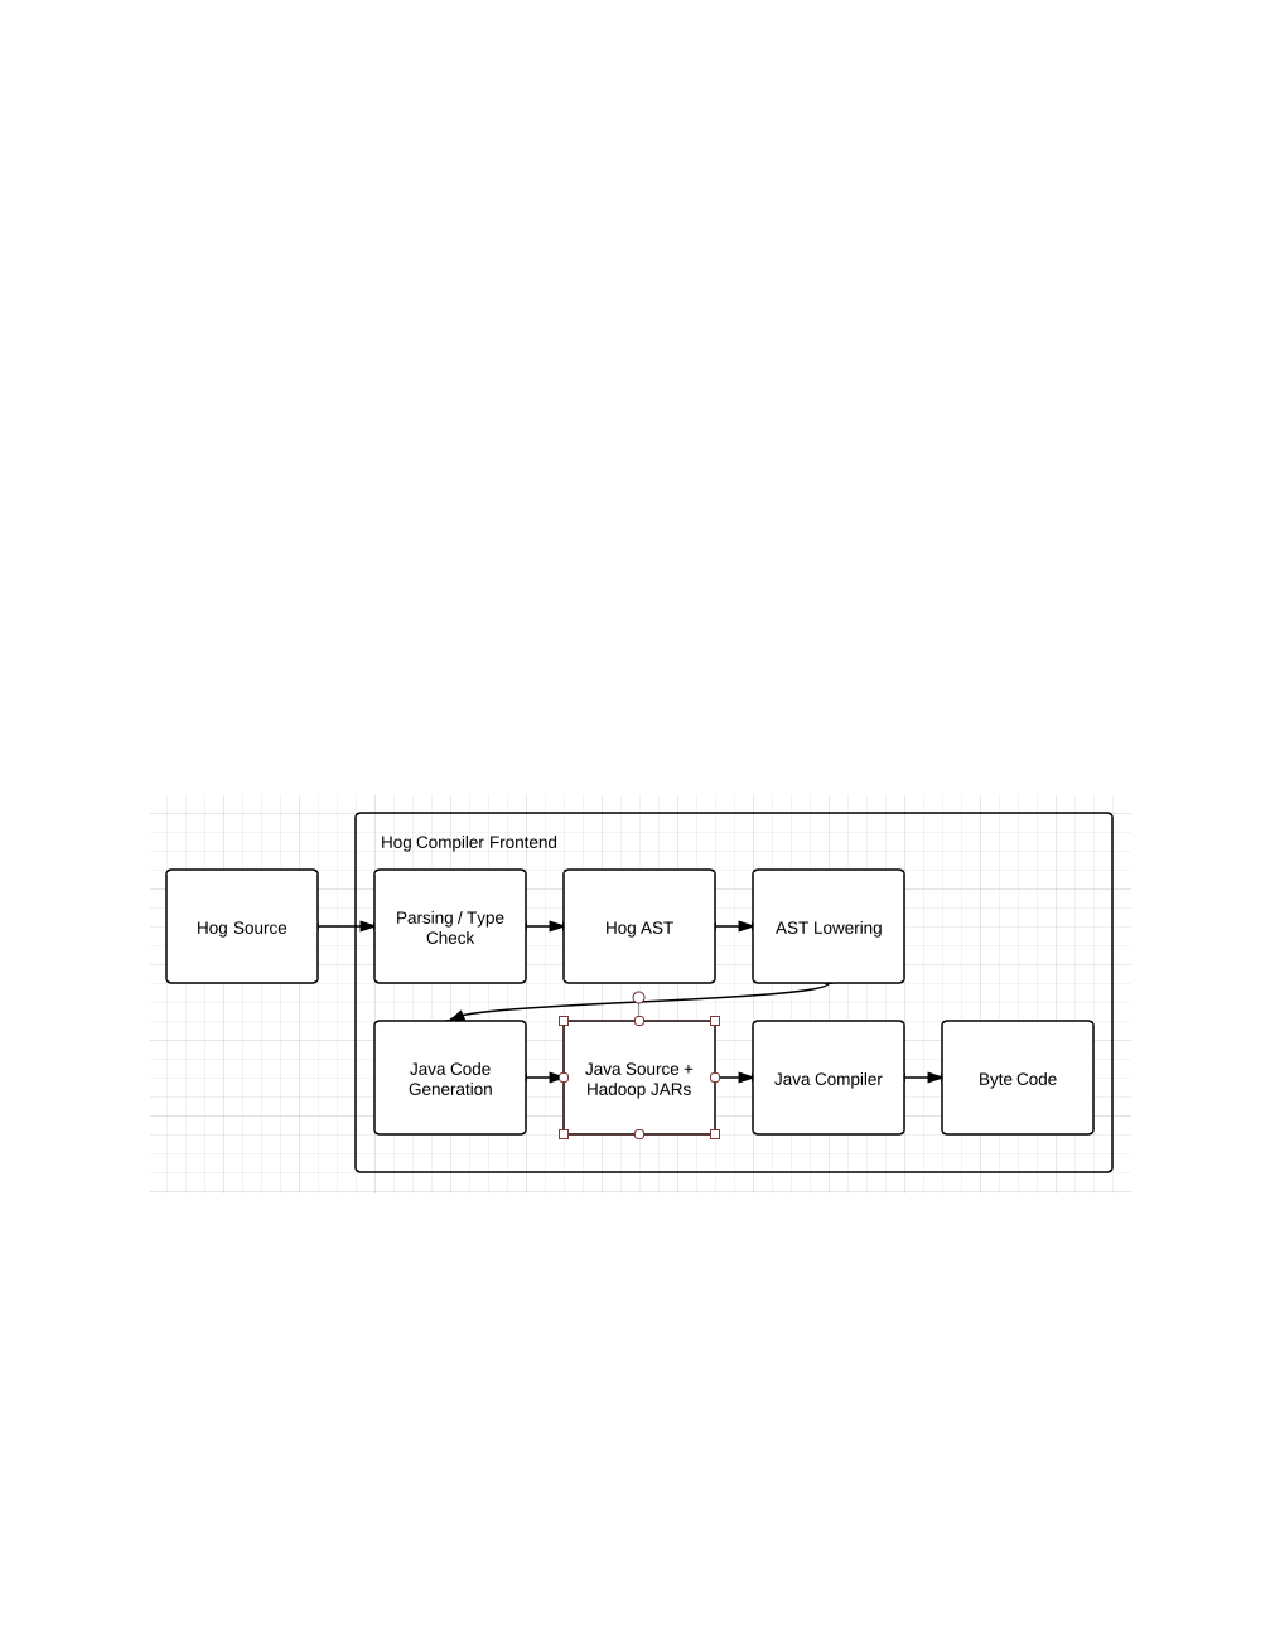
\includegraphics[width=1.0\textwidth]{img/hog_compiler.pdf}
  \caption{The overall structure of the Hog compiler.}
\end{figure}
\end{center}

\subsection{Usage} % (fold)
\label{sub:usage}

% subsection usage (end)

To build and run a Hog source file there is an executable script \tt hog
\rm that automates the compilation and linking steps for the user.

Usage: \tt hog [--hdfs|--local] job <job args> \rm
\begin{itemize}
  \item[] \tt --hdfs\rm: if job ends in '.hog' or '.java' and the file exists, link it against the hadoop JARFILE and then run it on HOST.
  \item[] \tt --local\rm: run on local host.
\end{itemize}

\subsection{Example} % (fold)
\label{sub:example}

\begin{verbatim}
hog --local WordCountJob.hog --input someInputFile.txt --output ./someOutputFile.csv
\end{verbatim}

This runs the \tt wordCount \rm job in \emph{local} mode (i.e. not on a Hadoop
cluster).

% subsection example (end)

% section linkage_and_i_o (end)

\section{Exception Handling} % (fold)
\label{sec:exception_handling}

Similar to other programming languages (Java, C++), Hog uses an exception model in
which an exception is thrown and can be caught by a catch block. Code should be
surrounded by a try block and then any exceptions occurring within the try block
will subsequently be caught by the catch block. Each try block should be
associated with at least one catch block. However, there can be multiple catch
blocks to handle specific types of exceptions. In addition, an optional finally
block can be added. The finally block will execute in all circumstances, whether
or not an exception is thrown. The structure of exception handling should be
similar to this, although there can be multiple catch blocks and the finally block
is optional:

\begin{quotation}
\tt try \{ \rm \\
\indent \indent \emph{expression} \\
\tt \indent \} catch ( \rm \emph{exception} \tt ) \rm \{ \\
\indent \indent \emph{expression} \\
\tt \indent \} finally \rm \{ \\
\indent \indent \emph{expression} \\
\tt \indent \}
\end{quotation}

Because the proper behavior of a Hog program is dependent on resources outside of
the language (i.e. the proper behavior of the user’s Hadoop software), there are
more sources exceptions in Hog than most general purpose languages. These sources
can be divided into three categories: \textbf{\emph{compile­time exceptions}},
\textbf{\emph{internal run­time exceptions}} and \textbf{\emph{external run­time
exceptions}}.

To throw an exception, a programmer uses the following pattern,

\begin{quotation}
\tt throw \rm \emph{exceptionType} \emph{exceptionMessage}
\end{quotation}

\noindent For example,

\begin{verbatim}
    if (a instanceof text and b instanceof int)
    throw TypeMismatchException "Cannot add a text and an int!"
\end{verbatim}

\subsection{Compile-time Exceptions} % (fold)
\label{sub:compile_time_exceptions}

The primary cause of most compile­time exceptions in Hog are syntax errors. Such
errors are unrecoverable because it is impossible for the compiler to properly
interpret the user program. Some compilers for other languages offer a limited
amount of compile­time error correction. Because Hog programs are often designed
to process gigabytes or terabytes of data at a time, the standard Hog compiler
offers no compile­time error correction. The assumption is that a user would
rather re­tool their program than risk the chance of discovering, only after hours
of processing, that the compilers has incorrectly assumed what the user meant. The
following are Hog compile­time exceptions:

\begin{itemize}
  \item[] \tt IncorrectArgumentException \rm
  
  Thrown when a derived-type object is instantiated with invalid parameters, or a function is called with invalid parameters.
  
  \item[] \tt TypeMismatchException \rm
  
  Thrown when a program attempts to carry out an operation on a variable of the wrong type (like adding a \tt text \rm and an
  \tt int \rm together). This exception can be generated at compile-time or run-time.
  
  \item[] \tt ProgramStructureException \rm
  
  Thrown when a Hog program does not follow the structure described earlier in section 2.1

  \item[] \tt NoSuchVariableException \rm
  
  Thrown when an attempt is made to use a variable that has not been declared yet.

  \item[] \tt NoSuchFunctionException \rm
  
  Thrown when a function is invoked that does not exist.

  \item[] \tt UnsupportedOperationException \rm
  
  Thrown when a variable invokes a function that is not supported for that type (i.e. when tokenize is invoked by a variable of type int).

  \item[] \tt UnreachableCodeException \rm

  Thrown when code is included in a part of a program that will never be executed (i.e. any code included after the emit function in the @Map and @Reduce sections).

  \item[] \tt RedundantDeclarationException \rm

  Thrown when a variable is redeclared in a program that it has previously been declared in.

\end{itemize}

% subsection compile_time_exceptions (end)

\subsection{Internal Run-time Exceptions} % (fold)
\label{sub:internal_run_time_exceptions}

Internal run­time exceptions include such problems as I/O exceptions (i.e. a specified file is not found on either the user’s
local file system or the associated Hadoop file system), type mismatch exceptions (i.e. a program attempts to place two
elements of different types into the same list) and parsing exceptions. The following are Hog internal rum­time exceptions:


\begin{itemize}
  \item[] \tt FileNotFoundException \rm
  
  Thrown when the the Hog program attempts to open a non-existent file.
  
  \item[] \tt FileLoadException \rm
  
  Thrown when an error occurs while Hog is attempting to read a file (e.g. the file is deleted while reading).
  
  \item[] \tt ArrayOutOfBoundsException \rm
  
  Thrown when a program tries to access a non-valid index of a \tt list\rm.
  
  \item[] \tt IncorrectArgumentException \rm
  
  Thrown when a derived-type object is instantiated with invalid parameters, or a function is called with invalid parameters.
  
  \item[] \tt TypeMismatchException \rm
  
  Thrown when a program attempts to carry out an operation on a variable of the wrong type (like adding a \tt text \rm and an
  \tt int \rm together).
  
  \item[] \tt HogMapFunctionException \rm
  
  Thrown when a map function receives a key, value pair of the wrong type.
  
  \item[] \tt HogReduceFunctionException \rm
  
  Thrown when a reduce function receives a key, value pair of the wrong type.
  
  \item[] \tt NullPointerException \rm
  
  Thrown whenever the value of a variable cannot be \tt null \rm (e.g. in \tt myList.get(i)\rm, if \tt i \rm is \tt null\rm,
  the operation with throw a \tt NullPointerException\rm).
  
  \item[] \tt ArithmeticException \rm
  
  Thrown whenever an arithmetic operation is attempted on non-numeric operands.
  
  \item[] \tt IOException \rm
  
  \item[] \tt InterruptedException \rm
  
  \item[] \tt ParseException \rm
\end{itemize}

% section internal_run_time_exceptions (end)

\subsection{External Run-time Exceptions} % (fold)
\label{sub:external_run_time_exceptions}


In Hog, if a compute-node throws any run-time exception
that causes the compute-node to crash or abort execution,
the tasks running on that node will be reassigned to other
compute-nodes automatically by the Hadoop runtime. There
will not be any data transferred between compute-nodes since
the Hadoop Distributed File System replicates the same data
across all compute-nodes.

In Hog, there is support for specifying a policy for retrying
method failures after an exception has been thrown, through the
interface RetryPolicy in Hadoop. The interface consists of one 
method:
     boolean shouldRetry(Exception e, int retries)  
which determines whether Hadoop should retry a method, and the
number of retries that have been attempted so far.

Hog also provides, through the Hadoop, prespecified retry policies:

\begin{enumerate}
  \item \tt RETRY\_FOREVER\rm: Keep trying forever. 
  \item \tt TRY\_ONCE\_DONT\_FAIL\rm: Try once, and fail silently for void methods,
  or by re-throwing the exception for non-void methods.
  \item \tt TRY\_ONCE\_THEN\_FAIL\rm: Try once, and fail by re-throwing the exception.
\end{enumerate}

% subsection external_run_time_exceptions (end)

% section exception_handling (end)

\section{Grammar} % (fold)
\label{sec:grammar}

\begin{verbatim}


declaration:
   declaration-specifiers

declaration-list:
   declaration
   declaration-list declaration

type-specifier: one of
   void int real bool text


selection-statement:
   if ( expression ) statement
   if ( expression ) statement else statement
   if ( expression ) statement elseif ( expression ) statement... else statement

   switch ( expression ) statement if ( expression ) statement
   if ( expression ) statement else statement
   if ( expression ) statement elseif ( expression ) statement... else statement
 
   switch ( expression ) statement

iteration-statement:  
   while ( expression ) statement
   for ( expression; expression; expression ) statement
   foreach ( expression in array or list) statement

@Functions:
   return­type function­name­1 (parameter­list) {
      exprlist 
   }
   returntype functionname2 (parameterlist){
      exprlist
   }

@Map: 
   (type key­name, type value­name) ­> (type, type) {
      .
      .
      .
  }

unary-operator:
[]

constant:

\end{verbatim}

% section grammar (end)


\end{document}
